\documentclass[type = bachelor]{whu-thesis}
\usepackage{textcomp,mathcomp}
\usepackage{siunitx}
\usepackage{chemfig}

\whusetup
  {
    info               =
      {
        title          = {金刚石氮-空位色心的\\电荷态调控和性质表征},
        title*         = {Modulation of Charge States and Characterization of Properties\\ in Nitrogen-Vacancy Centers of Diamond},
        student-number = {2020302192129},
        school         = {弘毅学堂},
        author         = {邹迪玮},
        author*        = {Diwei Zou},
        subject        = {学科},
        major          = {微电子科学与工程},
        advisor        = {周利 , 副教授;孙启超 , 研究员},
        direction      = {研究方向},
        date           = {2024/5},
        keywords       = {关键词 1 , 关键词 2 , 关键词 3 , 关键词 4 , 一个非常非常,非常非常长——的关键词 5},
        keywords*      = {key word 1 , key word 2 , key word 3 , key word 4 , {and a very very, very very long key word---the key word 5}},
      },
    style              =
      {
        graphics-path  = {{figures/}{data/}},
        list-of-figures,
        list-of-tables,
      },
    element            =
      {
        innovation     = {pages/innovation},
        abstract       = {pages/abstract},
        abstract*      = {pages/enabstract},
        bibliography   = {ref/refs_1}
      }
  }
\begin{document}

% Chapter 1

\chapter{金刚石中的氮-空位色心}

\section{金刚石}
金刚石是碳元素的一种常见的同素异形体,在晶体结构上,每一个碳原子被周围的四个碳原子包围并与之形成共价键,从而形成四面体的面心立方结构的晶体。金刚石中的碳原子紧密结合在一起,这样特殊的晶体结构和原子之间稳定的键合方式使得金刚石拥有很多物理和化学上的优异性质,如高硬度、高热导率、高折射率、高抗压强度、高化学稳定性、高电阻率、低热膨胀系数、低摩擦系数、低表面粗糙度、低吸附性等。这些优异的性质使得金刚石在很多领域都有着广泛的应用,如磨料、切割工具、磨料涂层、磁头、光学窗口、高功率激光器件、高频电子器件、生物医学器件等。

金刚石是最坚硬的天然形成的物质,其机械硬度高达 10000 \unit{\kilogram\per\milli\meter\squared},德拜温度高达1860 \unit{\kelvin},它的杨氏模量为1050 \unit{\GPa},有着22 \unit{\watt\per\centi\meter\per\kelvin}的热导率、较低的热展宽系数、较高的击穿电场强度(> 10 \unit{\mega\volt\per\centi\meter}),以及较强的载流子迁移率(对于电子为4500 \unit{\centi\meter\squared\per\volt},对于空穴为3800 \unit{\centi\meter\squared\per\volt})。对于纯净的金刚石而言,其密度为$\rho =$ 3.52 \unit{\g\per\cm},折射率$n =$ 2.39,同时有5.47 \unit{\electronvolt}的较宽带隙,这使其投射光谱范围非常广,从紫外波段(Ultraviolet,UV)到近红外波段(Near Infrared,IR)都可以覆盖到,外观高度透明纯净,拥有极高的透光率 \cite{mildren2013optical, lonvcar2013quantum}。

金刚石在结构上的稳定性使得其化学性质非常的不活跃,因此它几乎不能和大部分化学物质发生反应。所以金刚石有着极低的细胞毒性,使得其在生物、医学领域有着广泛的应用 \cite{schirhagl2014nitrogen,wu2016diamond}。同时,金刚石的化学稳定性也使得其在高温、高压、强腐蚀性环境下有着很好的稳定性,因此金刚石也被广泛应用于高温、高压、强腐蚀性环境下的传感器、探测器等器件中 \cite{umezawa2012high, jayaraman1983diamond}。

由于金刚石晶体的结构非常的整齐和规则,在自然情况下,只有很少一部分的杂质会存在于金刚石晶体中,并参与形成晶格结构。自然界中常见的最主要的金刚石中的杂质是氮和硼元素,因此金刚石可以根据杂质的种类和含量分为不同的类型,主要有两种大类:type \uppercase\expandafter{\romannumeral1}和type \uppercase\expandafter{\romannumeral2},在其中又可以分为四个子类:type \uppercase\expandafter{\romannumeral1}a、type \uppercase\expandafter{\romannumeral1}b、type \uppercase\expandafter{\romannumeral2}a、type \uppercase\expandafter{\romannumeral2}b \cite{breeding2009type}。在这些分类中,type \uppercase\expandafter{\romannumeral1}型的金刚石中主要含有氮元素杂质,type \uppercase\expandafter{\romannumeral1}a型金刚石中的氮元素含量较高,最多有3000 ppm(parts per million,即百万分之一);而type \uppercase\expandafter{\romannumeral1}b型金刚石中的氮元素含量稍低,一般情况下不到500 ppm。由于空气中广泛存在的氮气和土壤中各种各样的氮元素,在自然界中形成的金刚石通常为type \uppercase\expandafter{\romannumeral1}a或者\uppercase\expandafter{\romannumeral1}b。对于type \uppercase\expandafter{\romannumeral2}型的金刚石而言,氮元素的含量远远小于type \uppercase\expandafter{\romannumeral1}型金刚石,通常低于20 ppm。其中,type \uppercase\expandafter{\romannumeral2}b型金刚石中的硼元素杂质含量要高于type \uppercase\expandafter{\romannumeral2}a型。Type \uppercase\expandafter{\romannumeral2}型金刚石的含量极其稀少,而且很少能在自然界中被发现。在科学研究中,type \uppercase\expandafter{\romannumeral2}型金刚石由于其晶体纯净的性质,有着各种各样独特的应用场景。对于科学研究而言,为了保证金刚石样品性质的一致性和实验的可重复性,高纯度和可控掺杂的人造金刚石生长合成技术应运而生 \cite{sumiya1997crystalline, spitsyn1981vapor, gracio2010diamond}。

\subsection{人工合成生长金刚石}
目前主流的人造金刚石样品合成技术主要分为两种,一种是高温高压方法(High Pressure High Temperature,HPHT)和化学气相沉积法(Chemical Vapor Deposition,CVD)。对于HPHT方法而言,其原理主要是模仿天然金刚石在地壳中的形成过程,将碳元素另一种常见的同素异形体石墨的晶体结构在极端的超高温超高压环境下(温度在\SI{1400}{\degreeCelsius}左右,压强在\SI{5.5}{\GPa}左右),通过金属触媒粉的催化作用,转换成具有$sp^3$杂化轨道的金刚石晶体结构 \cite{dossa2023analysis}。HPHT方法使得人类可以在工业上大规模高效率地生产type \uppercase\expandafter{\romannumeral1}型金刚石,但是由于空气中大量的氮气存在,HPHT方法难以生产高纯度低杂质含量的type \uppercase\expandafter{\romannumeral2}型金刚石。由此,为了制备高纯度和可控掺杂的实验级金刚石样品,化学气相沉积的方法逐渐受到科学家们的关注和广泛使用。

CVD方法是一种铜质外延的生长过程,需要在金刚石晶种基面上生长新的金刚石\cite{isberg2002high,isberg2002high}。因此,对于生长出来的晶体,其质量主要取决于晶种的种类和取向,而在非金刚石晶种表面生长会导致生长出有许多单晶金刚石各向同性紧密结合形成的多晶金刚石晶体\cite{mildren2013optical, jahnke2012long}。如果想要形成科学实验中可用的单晶金刚石,就必须用单晶金刚石作为晶种来进行CVD生长。在实际生长的过程中,科学家们通常用{100}取向的晶种衬底来保证尽可能少的生长缺陷\cite{gicquel2001cvd}。

在CVD方法生长金刚石的过程中,除了晶种之外,碳元素源也是比较重要的一个因素。通常情况下,碳元素主要来自于烃类气体,甲烷\chemfig{CH_4}和氢气\chemfig{H_2}的混合气体就是在实验合成的过程中较为理想易得的碳源。对于CVD生长金刚石的过程而言,这些碳源气体需要通过不同的方法来激活,常见的方法有通过热丝(hot filament)或者微波等离子体(microwave plasma),其中微波等离子体气相沉积(Microwave Plasma Chemical Deposition,MPCVD)的方法是生长type \uppercase\expandafter{\romannumeral2}型金刚石最有效的方法\cite{robins1990line, nemanich2014cvd}。在微波等离子体激活后,碳源气体内部形成许多高度反应性的自由基(reactive radicals),活跃的氢自由基(H$\cdot$)有两个重要的功能,一个是终止了已经生长的金刚石表面,从而防止具有$sp^2$杂化轨道的石墨碳原子;其次氢原子可以刻蚀掉已经生成的具有$sp^2$杂化轨道的石墨碳原子,从而在晶种沉底表面上提供悬垂的$sp^3$化学键,使其能够和已经极化的甲基自由基(CH$_3\cdot$)轻松结合,使得单晶金刚石能在沉底表面逐渐生长\cite{denisenko2010surface}。在生长的过程中,各种参数同样十分重要,例如生长腔内压强、温度、气体流速、微波功率等因素决定了生长出来的金刚石的各种性质,使其适用于不同的应用场景。本人于2021年的时候提出了一种n型共掺杂金刚石半导体材料制备的多尺度耦合仿真方法,通过宏观-介观-微观三个尺度的相互耦合,调整MPCVD方法生长金刚石过程中的各种参数,来提高特定用途金刚石的生长合成效率\cite{CN113096749B}。

\subsection{金刚石晶体结构}
金刚石晶体是由每个碳原子和周围四个相邻的碳原子结合,生成四个共价键组成的正四面体结构,其晶格常数为$a_0 = 3.567$ \unit{\angstrom}。金刚石晶体可以看成是两个面心立方晶体的嵌套,其中一个面心立方晶体在三维空间的三个轴上上相对于另一个移动了$\frac{a_0}{4}$,原点从$(0, 0, 0)$移动到了$(\frac{a_0}{4}, \frac{a_0}{4}, \frac{a_0}{4})$。这样的晶体结构使得金刚石非常的坚硬,每一个晶胞中包含着8个碳原子,每一个碳原子的核外电子都呈现$sp^3$杂化轨道结构,和相邻的碳原子形成长度为1.44 \unit{\angstrom}的共价键,其晶体结构见图1.1。

\begin{figure}[h]
  \centering
  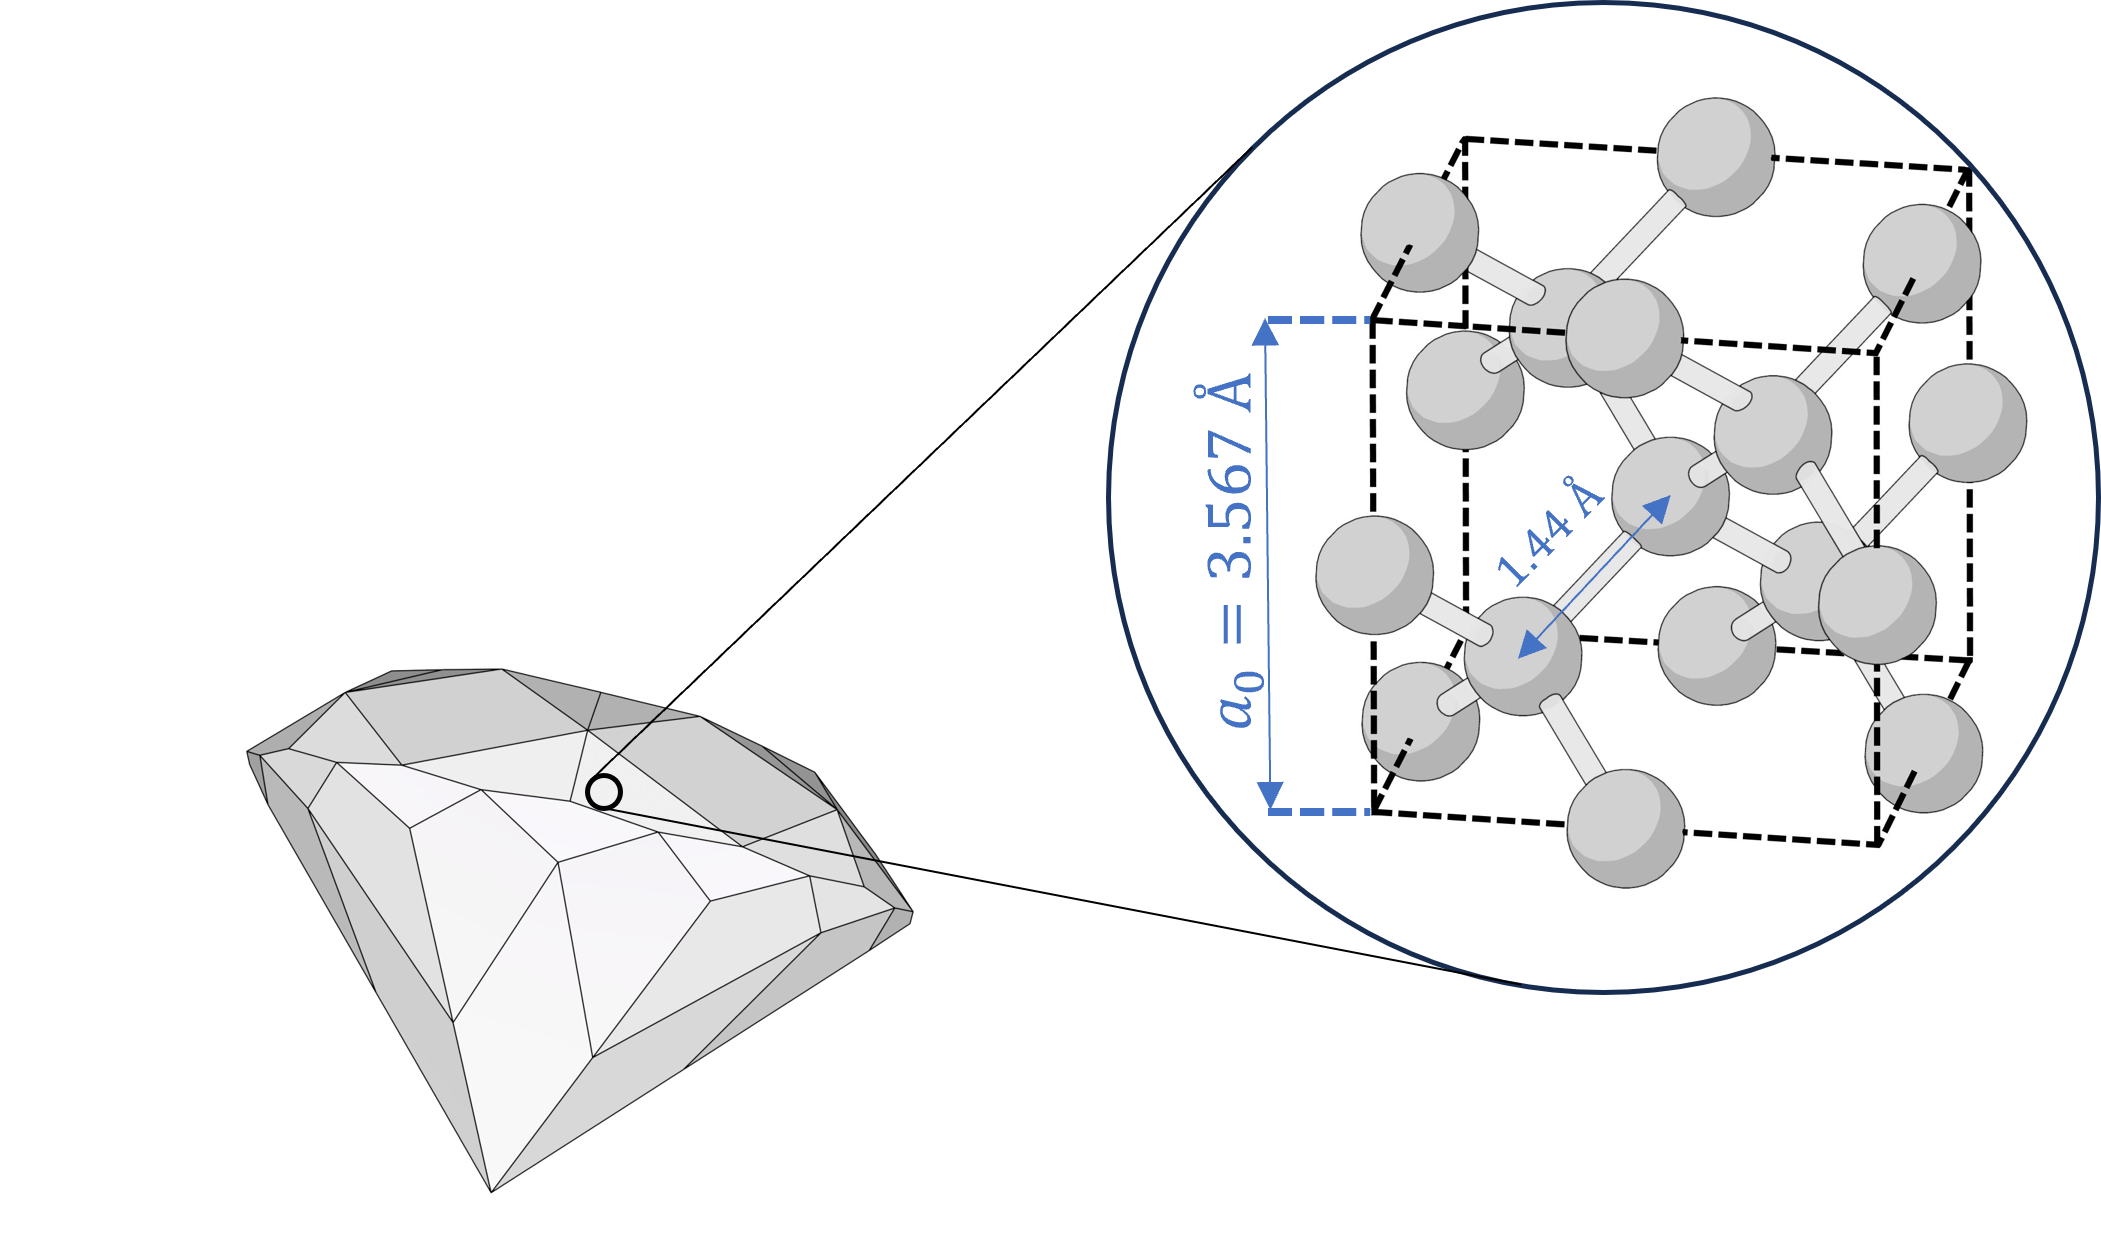
\includegraphics[width=0.7\textwidth]{figures/Chapter 1/Diamond Lattice.png}
  \caption{金刚石及其晶胞结构}
  \label{fig:Diamond Lattice}
\end{figure}

然而,在金刚石晶体合成或生长的过程中,晶格缺陷会不可避免的出现,它们会对金刚石的性质产生各种各样的影响,尤其是电子结构产生较大的影响\cite{jelezko2006single, nebel2003electronic}。金刚石晶体中最常见的晶格缺陷是空位(vacancy),这是一种本征晶格缺陷,源于金刚石的中的单个碳原子在其原本的晶格结构上的缺失,每一个孤立的空位可以吸收741 nm的光子,有着高浓度空位的金刚石在一定条件下会呈现蓝绿色的色调,因此金刚石晶体结构中的空位缺陷也被称为色心(color centers),如图1.2所示\cite{waldermann2007creating, kiflawi2007electron}。

\begin{figure}
  \centering
  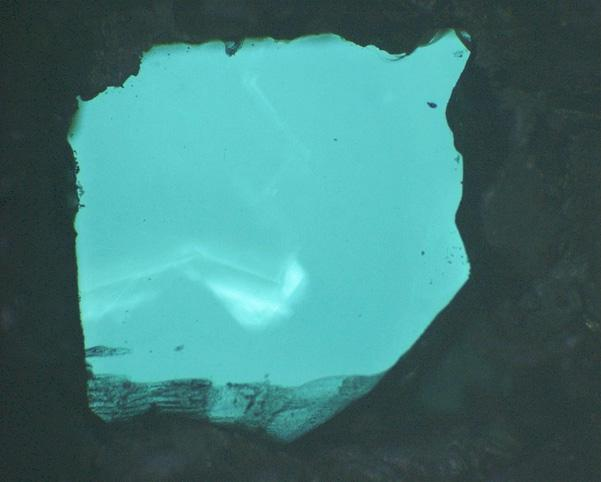
\includegraphics[width=0.7\textwidth]{figures/Chapter 1/Color Center.jpg}
  \caption{电子辐照的type \uppercase\expandafter{\romannumeral1}a型金刚石样品显微图片,浅色区域的空位和氮浓度较低,样品尺寸为\(1\times1\times0.5 \, \mathrm{mm^3}\)。}
  \label{fig:Color Center}
\end{figure}

\subsection{金刚石色心}
金刚石是一种宽禁带半导体,实验上测得其价带(valence band,VB)和导带(conduction band,CB)之间的带隙宽度大约为5.5 \unit{\eV} \cite{mildren2013optical,cheng2023bandgap,wort2008diamond}。尽管纯净的金刚石呈现无色透明的质地,可以透过的波长范围从UV到IR,但是由于晶格中存在的缺陷或者杂质,使得金刚石体系的带隙之中会出现额外的能级结构,其中的一些能级结构具有活跃的光学性质。因此,这些缺陷结构可以吸收可见光,并在缺陷浓度足够高的时候,使得金刚石材料呈现出特定的颜色,比如高浓度的硼元素会使金刚石呈现蓝色,镍元素相关的缺陷会让金刚石呈现棕色。目前人类已知金刚石中的涉及到光学跃迁性质的荧光缺陷有超过100种,这些缺陷都可以被称为色心\cite{koizumi2008physics,jelezko2006single}。许多的色心都和氮元素杂质有关,因为氮元素是金刚石中最常见的元素,高浓度的氮元素掺杂会使得金刚石呈现黄色的色泽\cite{breeding2020naturally, zaitsev2016spectroscopic}。

金刚石色心种的缺陷能级和电子结构之间的光学跃迁过程可以被人为地进行激光调控,在这个过程中会有不同的激发机理,取决于色心相关的缺陷能级的性质,如图1.3所示。比如,激光的光子可以将缺陷能级的电子激发到导带之中(见图1.3a \uppercase\expandafter{\romannumeral1}所示),或者将电子从夹带激发到缺陷能级见图1.3a \uppercase\expandafter{\romannumeral2所示}。另一种常见的情况是在带隙中有多个缺陷能级的情况,激光可以将电子从一个缺陷能级激发到另一个缺陷能级(见图1.3b所示),这种跃迁的方式相较于电子在缺陷能级和导带(或价带)之间相互跃迁能为高效和可控\cite{gali2011time,gali2012excitation}。在各种各样的色心之中,氮-空位色心(Nitrogen-Vacancy Center)在近些年来被许多科学家所广泛研究,其在532 nm激光的激发下会发出红色的荧光\cite{doherty2013nitrogen}。

\begin{figure}
  \centering
  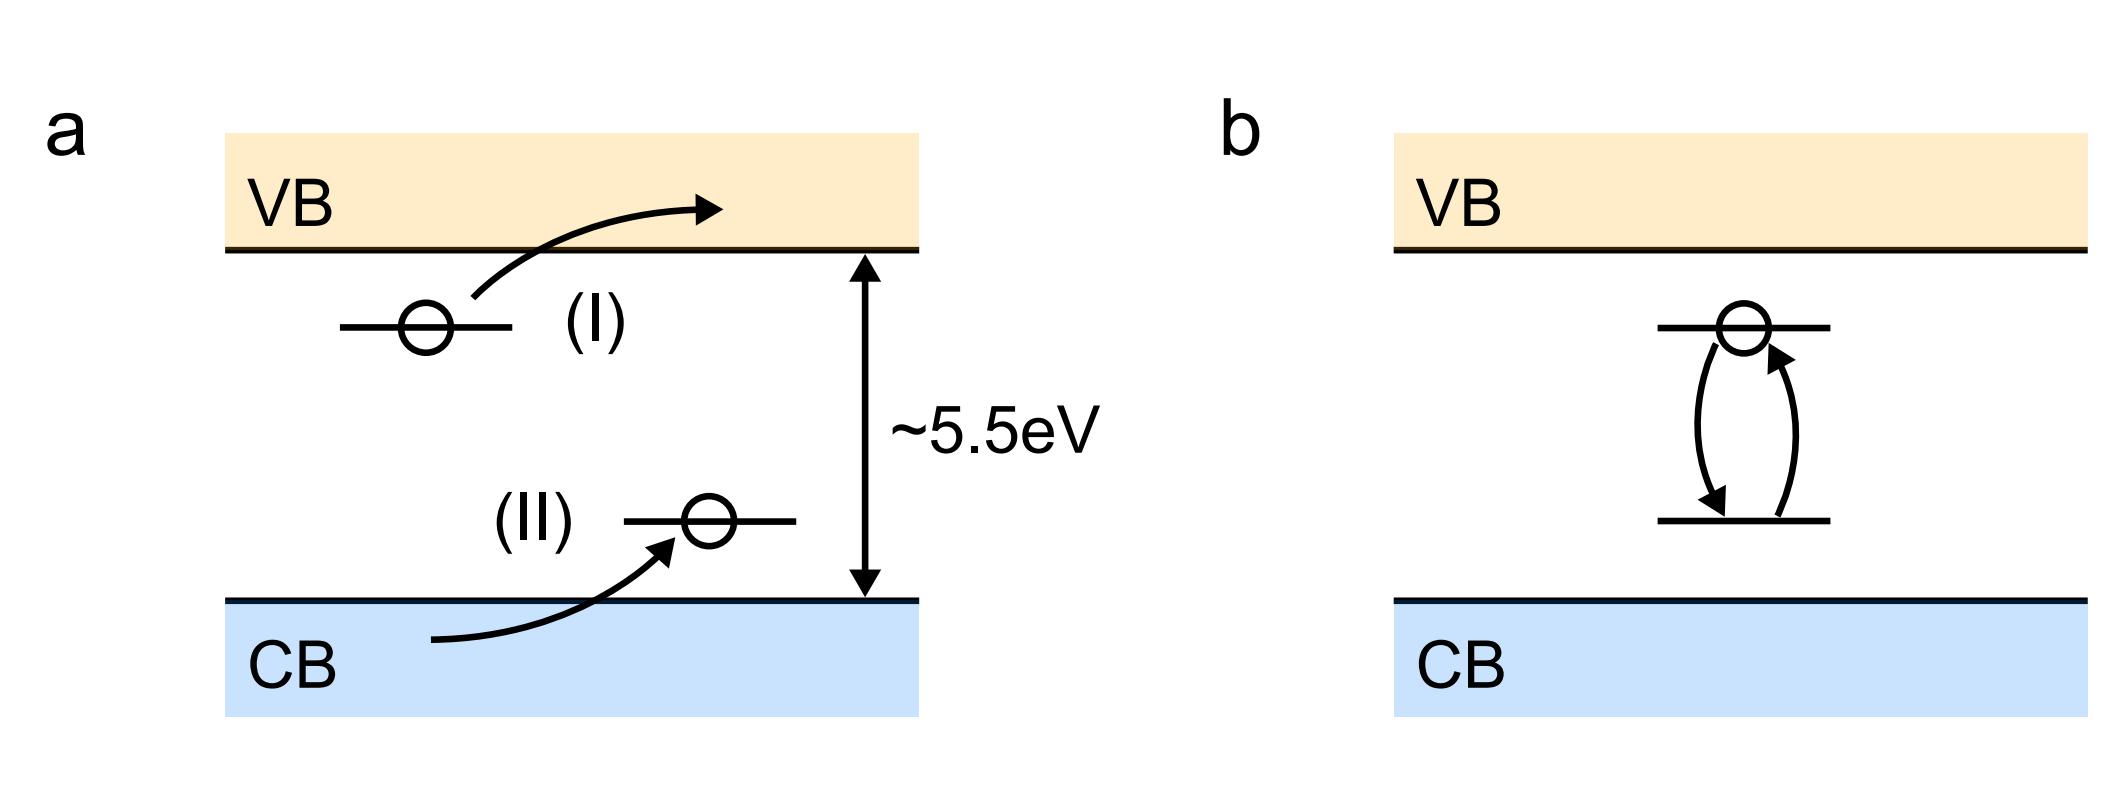
\includegraphics[width=0.7\textwidth]{figures/Chapter 1/Optical Transition.png}
  \caption{含有缺陷的金刚石电子结构。(a)带隙之间的施主和受主能级会使电子发生在价带和缺陷能级(\uppercase\expandafter{\romannumeral1})或缺陷能级和导带(\uppercase\expandafter{\romannumeral2})之间的光学跃迁。(b)电子在施主和受主能级之间的光学跃迁}
  \label{fig:Optical Transition}
\end{figure}


\section{论文题目的写法}
论文题目应简明扼要地反映论文工作的主要内容,力求精炼、准确,切忌笼统。论文题目是对研究对象的准确、具体描述,一般要在一定程度上体现研究结论,因此,论文题目不仅应告诉读者这本论文研究了什么问题,更要告诉读者这个研究得出的结论。例如:“在事实与虚构之间:梅乐、卡彭特、沃尔夫的新闻观”就比“三个美国作家的新闻观研究”更专业、更准确。

\section{摘要的写法}
论文摘要是对论文研究内容的高度概括,应具有独立性和自含性,即应是一篇简短但意义完整的文章。通过阅读论文摘要,读者应该能够对论文的研究方法及结论有一个整体性的了解,因此摘要的写法应力求精确简明。论文摘要应包括对问题及研究目的的描述、对使用的方法和研究过程进行的简要介绍、对研究结论的高度凝练等,重点是结果和结论。

论文摘要切忌写成全文的提纲,尤其要避免“第 1 章……;第 2 章……;……”这样的陈述方式。

\section{引言的写法}
一篇学位论文的引言大致包含如下几个部分:1.~问题的提出;2.~选题背景及意义;3.~文献综述;4.~研究方法;5.~论文结构安排。
\begin{itemize}
    \item 问题的提出:要清晰地阐述所要研究的问题“是什么”。\footnote{选题时切记要有“问题意识”,不要选不是问题的问题来研究。}
    \item 选题背景及意义:论述清楚为什么选择这个题目来研究,即阐述该研究对学科发展的贡献、对国计民生的理论与现实意义等。
    \item 文献综述:对本研究主题范围内的文献进行详尽的综合述评,“述”的同时一定要有“评”,指出现有研究状态,仍存在哪些尚待解决的问题,讲出自己的研究有哪些探索性内容。
    \item 研究方法:讲清论文所使用的学术研究方法。
    \item 论文结构安排:介绍本论文的写作结构安排。
\end{itemize}

\section{正文的写法}
本部分是论文作者的研究内容,不能将他人研究成果不加区分地掺和进来。已经在引言的文献综述部分讲过的内容,这里不需要再重复。各章之间要存在有机联系,符合逻辑顺序。

\section{结论的写法}
结论是对论文主要研究结果、论点的提炼与概括,应精炼、准确、完整,使读者看后能全面了解论文的意义、目的和工作内容。结论是最终的、总体的结论,不是正文各章小结的简单重复。结论应包括论文的核心观点,主要阐述作者的创造性工作及所取得的研究成果在本领域中的地位、作用和意义,交代研究工作的局限,提出未来工作的意见或建议。同时,要严格区分自己取得的成果与指导教师及他人的学术成果。

在评价自己的研究工作成果时,要实事求是,除非有足够的证据表明自己的研究是“首次”“领先”“填补空白”的,否则应避免使用这些或类似词语。

\section{各节一级标题}
我是内容

\subsection{各节二级标题}
你是内容

\subsubsection{各节三级标题}
他是内容

\paragraph{四级标题}
内容内容

\subparagraph{五级标题}
内容内容

\section{字体样式}
宋体\quad \textbf{粗体}\quad \textit{斜体}\quad \textbf{\textit{粗斜体}}。

{\heiti 黑体\quad \textbf{粗体}\quad \textit{斜体}\quad \textbf{\textit{粗斜体}}}。

{\fangsong 仿宋\quad \textbf{粗体}\quad \textit{斜体}\quad \textbf{\textit{粗斜体}}}。

{\kaishu 楷书\quad \textbf{粗体}\quad \textit{斜体}\quad \textbf{\textit{粗斜体}}}。

Serif\quad \textit{Italic}\quad \textbf{Bold}\quad \textbf{\textit{BoldItalic}}

{\sffamily Sans\quad \textit{Italic}\quad \textbf{Bold}\quad \textbf{\textit{BoldItalic}}}

{\ttfamily Mono\quad \textit{Italic}\quad \textbf{Bold}\quad \textbf{\textit{BoldItalic}}}

\end{document}